% Cuerpo equivalente actualizado al 14 de octubre de 2026. Requiere graphicx, amsmath, booktabs, colores/macro pct de la fuente y las carpetas figures. Integre las referencias morris1991 y campolongo2007.
\section{Qué se puede concluir del estudio}
La pregunta estudiada es cómo cambian las frecuencias del modelo existente al modificar propiedades de las palas y velocidad del rotor. La respuesta depende del grupo modal. Entre los \emph{tres factores comparados}, la masa e inercia de palas tienen la mayor influencia media en las respuestas 3, 4+5, 8+9 y 10+11; la velocidad del rotor tiene la mayor influencia media en 6+7. Esta clasificación se refiere a un dominio exploratorio de factores entre 0.90 y 1.10.

Se completaron cuarenta trayectorias Morris: 160 evaluaciones del diseño y diez controles numéricos, todas convergidas. El diseño visitó 58 combinaciones diferentes; sus repeticiones se conservaron. Se aceptaron catorce indicadores de influencia media de frecuencia. Su cambio entre veinte y cuarenta trayectorias fue menor de 1\pct. Se aceptaron dos indicadores de dispersión, asociados a masa y rigidez en 10+11. Estas observaciones constituyen evidencia de sensibilidad del modelo numérico; no son una validación experimental ni una probabilidad de respuesta.

Una forma útil de presentar la contribución es: \emph{se obtuvo un cribado de influencia por grupo modal, con seguimiento de formas, actualización del equilibrio y filtros explícitos de ruido y estabilización}. El aporte científico incluye los signos opuestos del efecto del giro, la compensación parcial masa--rigidez y la identificación de respuestas cuya sensibilidad aún no puede resolverse.


El 14 de octubre se completó la rejilla de 64 combinaciones reutilizando 58 puntos y resolviendo seis faltantes. Se añadieron tres controles numéricos. Los nueve casos nuevos convergieron, sin cambios de rangos ni formulación. El contraste masa--rigidez de 10+11 supera la envolvente empírica en las cuatro velocidades examinadas.

\section{Qué se varió y qué representa el modelo}
Se denotan los factores por $\xi_\rho$ (masa e inercias de palas), $\xi_K$ (rigideces seccionales de palas) y $\xi_\Omega$ (velocidad del rotor). Su nominal es uno. El subíndice $\rho$ expresa un escalamiento compatible con cambio de densidad a geometría fija; no identifica una densidad experimental única de las palas.

\begin{center}\small
\begin{tabular}{p{2cm}p{7.1cm}p{3.7cm}}
\toprule Factor & Cambio consistente & Intervalo aprobado \\ \midrule
$\xi_\rho$ & Masa por longitud e inercias seccionales de las tres palas, con geometría y centroides fijos. & 0.90--1.10 \\
$\xi_K$ & Rigideces axial, de cortante, torsional y de flexión de las palas, escaladas conjuntamente. & 0.90--1.10 \\
$\xi_\Omega$ & Velocidad prescrita alrededor del eje del rotor, constante en cada caso. & 10.8--13.2 rpm \\
\bottomrule
\end{tabular}
\end{center}
Los rangos son escenarios aprobados, no límites de fabricación medidos. Los restantes parámetros conservan sus valores en esta campaña. Por ello, la clasificación global no compara exhaustivamente palas, torre, cimentación y conexiones.

\begin{figure}[htbp]
\centering
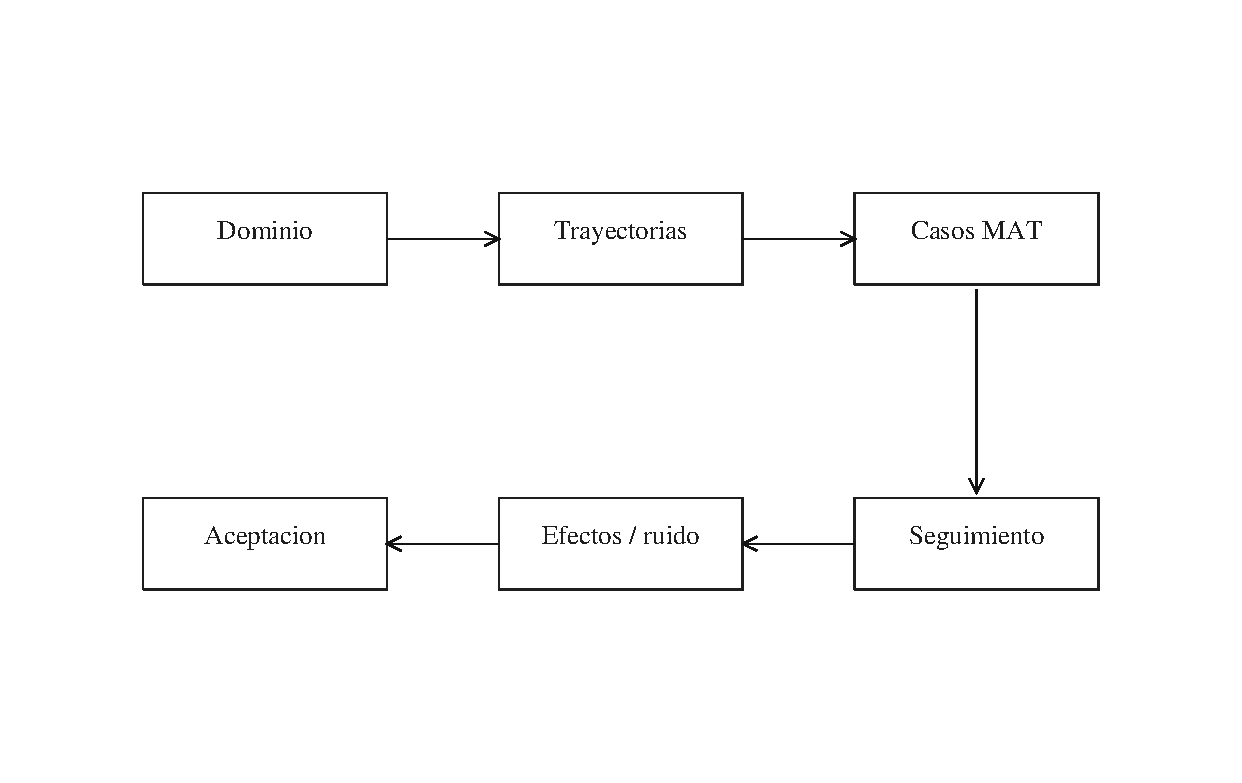
\includegraphics[width=.96\linewidth,height=.40\textheight,keepaspectratio]{figures/tecplot/morris_proceso.pdf}
\caption{Flujo del posprocesamiento de sensibilidad: dominio exploratorio, trayectorias, casos almacenados, seguimiento, efectos frente al ruido y aceptación. Cada caso es un equilibrio independiente a azimut congelado; la sensibilidad total incluye el cambio del equilibrio y de los operadores. El giro se prescribe alrededor del eje 129--130, sin guiñada nominal.}\label{fig:proceso}
\end{figure}

\section{Cómo leer las frecuencias y los grupos}
Sea $\boldsymbol q$ el vector de coordenadas perturbadas alrededor del equilibrio y $t$ el tiempo. Los operadores efectivos de masa, velocidad y tangente se denotan por $\mathsf M$, $\mathsf D$ y $\mathsf K$. La parte homogénea de la linealización congelada se escribe
\begin{equation}
\mathsf M\ddot{\boldsymbol q}+\mathsf D\dot{\boldsymbol q}+\mathsf K\boldsymbol q=\boldsymbol 0.
\end{equation}
La matriz $\mathsf D$ reúne amortiguamiento, efectos giroscópicos y transporte; sus términos no representan todos disipación material. La tangente $\mathsf K$ incluye las contribuciones implementadas del equilibrio y del giro, con las transformaciones cinemáticas correspondientes.

Sean $\lambda$ una raíz compleja y $\boldsymbol\phi$ su forma modal. Con $\boldsymbol q\propto\boldsymbol\phi\exp(\lambda t)$ se obtiene el problema cuadrático
\begin{equation}
[\lambda^2\mathsf M+\lambda\mathsf D+\mathsf K]\boldsymbol\phi=\boldsymbol 0.
\end{equation}
Se definen frecuencia amortiguada $f_d=|\operatorname{Im}\lambda|/(2\pi)$ [Hz], crecimiento $\gamma=\operatorname{Re}\lambda$ [s$^{-1}$] y razón de amortiguamiento $\zeta=-\operatorname{Re}\lambda/|\lambda|$. La frecuencia mide oscilaciones por segundo; el crecimiento mide evolución de la envolvente. Una frecuencia que aumenta no implica, por sí sola, mayor estabilidad.

Las etiquetas 6+7 o 10+11 identifican conjuntos de ramas de la referencia, no posiciones que se vuelvan a ordenar por frecuencia en cada caso. Se correlacionan formas complejas en el espacio físico con la masa nominal y se comprueban subespacios cuando hay raíces próximas. La respuesta de un grupo es la \emph{media de las frecuencias de sus ramas}; no constituye una nueva forma modal individual. Las ramas 4 y 5 se agruparon por su proximidad en parte del dominio ampliado. La rama 12 toca la frontera del conjunto seguido y se excluye de los estimadores; sus vecinos del espectro calculado impiden tratarla como grupo cerrado.

\begin{center}\small
\begin{tabular}{lrlp{3cm}}
\toprule Respuesta & $f_{d,0}$ [Hz] & Mayor influencia media & Signo aceptado del giro \\ \midrule
3 & 0.231 & Masa/inercia & $-$ \\
4+5 & 0.409 & Masa/inercia & No resuelto \\
6+7 & 0.587 & Velocidad & $+$ \\
8+9 & 0.844 & Masa/inercia & $+$ \\
10+11 & 1.225 & Masa/inercia & $+$ \\

\bottomrule
\end{tabular}
\end{center}
Aquí $f_{d,0}$ es la frecuencia nominal individual o media del grupo. El giro tiene efecto positivo en tres grupos y negativo en la rama 3. Su efecto en 4+5 permanece no resuelto frente al ruido. Una ausencia de aceptación no significa ausencia de influencia física.

\section{Cómo funciona Morris en este estudio}
Sea $x_i\in[0,1]$ la coordenada normalizada del factor $i$. Se aplica $\xi_i=\ell_i+(u_i-\ell_i)x_i$, donde los límites son $\ell_i=0.90$ y $u_i=1.10$. Se generan trayectorias aleatorias sobre cuatro niveles, con semilla 6706 y paso firmado $\Delta x_i$ de magnitud $2/3$ \cite{morris1991}. Cada segmento cambia un factor y conserva los otros dos. A lo largo de cuarenta trayectorias, ese cambio se observa en diferentes combinaciones del dominio.

\begin{figure}[htbp]
\centering
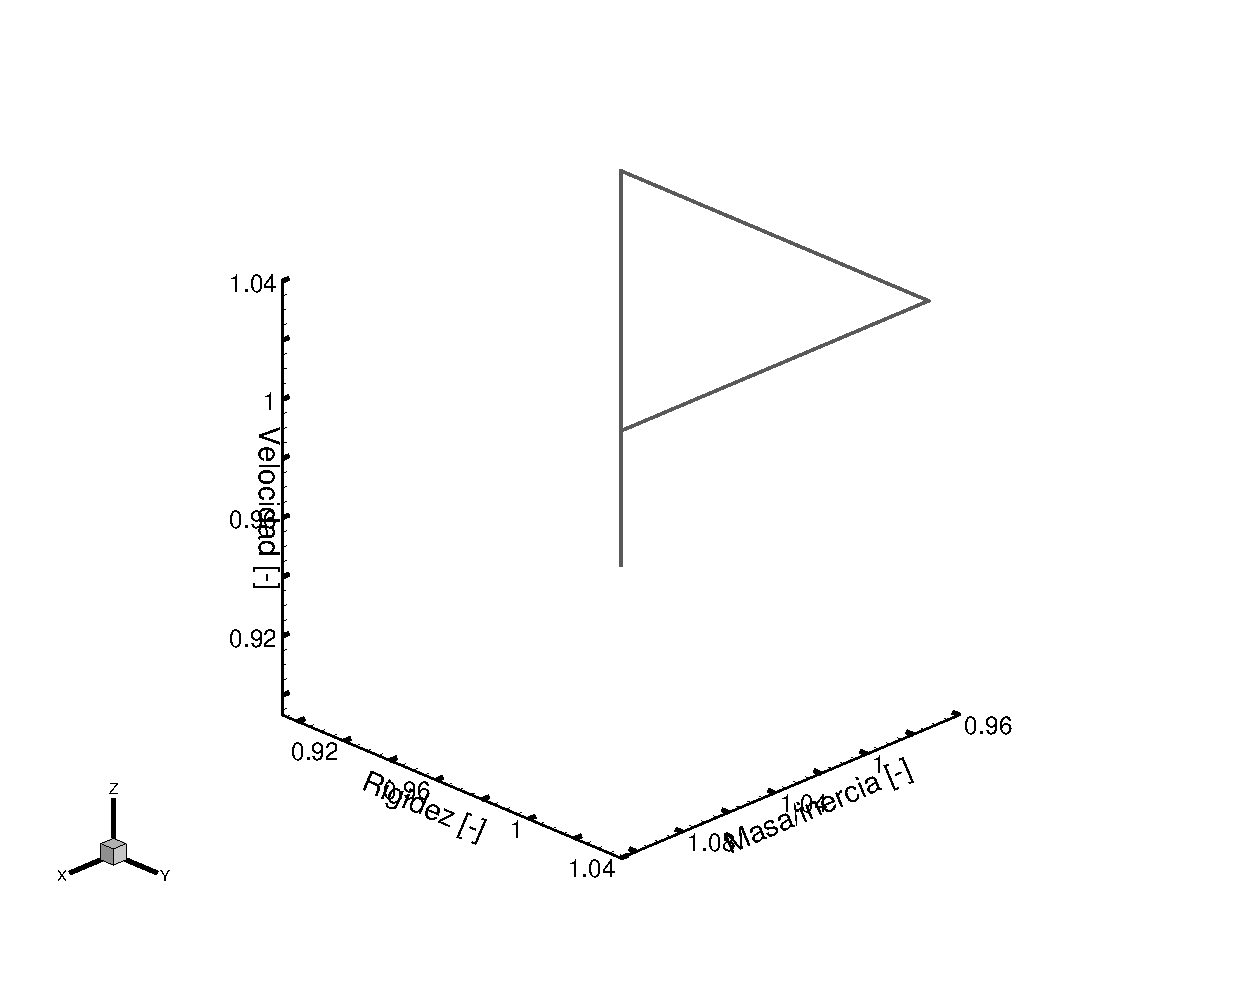
\includegraphics[width=.96\linewidth,height=.40\textheight,keepaspectratio]{figures/tecplot/morris_trayectoria.pdf}
\caption{Primera trayectoria ejecutada en los tres factores del diseño. Cada arista modifica un solo factor. Los segmentos unen casos almacenados y no describen una evolución temporal del rotor.}\label{fig:trayectoria}
\end{figure}
\begin{figure}[htbp]\centering
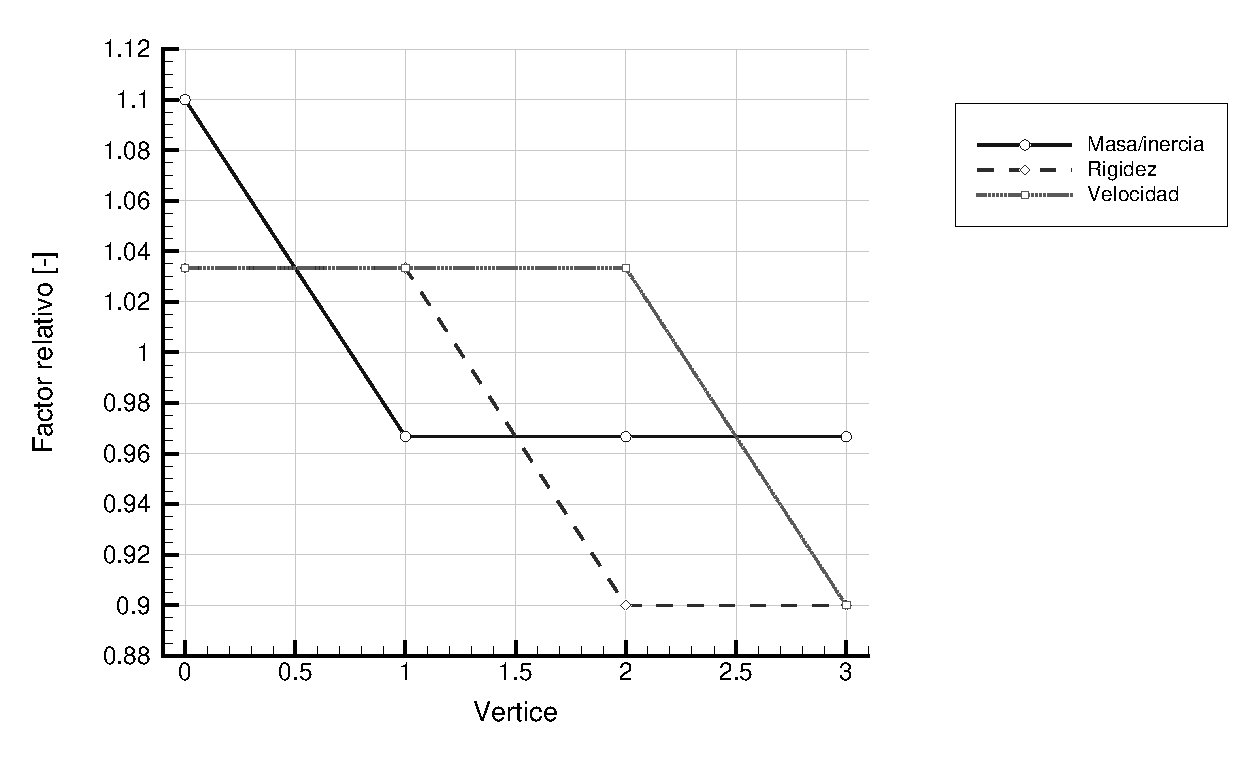
\includegraphics[width=.96\linewidth,height=.40\textheight,keepaspectratio]{figures/tecplot/morris_trayectoria_factores.pdf}
\caption{Factores por vértice de la primera trayectoria, en su orden de evaluación. Los símbolos identifican masa/inercia de palas, rigidez y velocidad. El eje horizontal indica vértices del diseño, no tiempo físico.}\label{fig:trayectoria-factores}\end{figure}

El tamaño del paso del factor es $|\Delta\xi_i|=0.20(2/3)=0.13333$. Aunque los puntos están dentro de $\pm10\pct$ respecto del nominal, cada secante atraviesa 13.333\pct\ del factor nominal. Esta es una razón para distinguir un efecto elemental de una derivada infinitesimal.

Sea $y$ una respuesta escalar y $s_y$ su escala nominal fija. Para frecuencia se usa $s_y=f_{d,0}$; para crecimiento, la media nominal de $|\lambda|$; para amortiguamiento, $\max(|\zeta_0|,0.01)$. El efecto elemental de la trayectoria $j$ es
\begin{equation}
EE_i^{(j)}=\frac{y_{\rm fin}^{(j)}-y_{\rm inicio}^{(j)}}{\Delta x_i^{(j)}s_y}.
\end{equation}
El signo del paso se conserva. Por ejemplo, en la primera arista del grupo 10+11 se \emph{reduce} $\xi_\rho$ de 1.10 a 0.9667 y la frecuencia \emph{aumenta} de 1.203767 a 1.263304 Hz:
\begin{equation}
EE_\rho^{(1)}=\frac{1.263304-1.203767}{(-2/3)(1.225430)}\simeq-0.07288.
\end{equation}
Su signo negativo describe la disminución de frecuencia al \emph{aumentar} masa/inercia. Este ejemplo proviene de casos almacenados; no es una simulación adicional.

Para $r$ trayectorias se calculan
\begin{align}
\mu_i&=\frac{1}{r}\sum_{j=1}^r EE_i^{(j)},&
\mu_i^*&=\frac{1}{r}\sum_{j=1}^r |EE_i^{(j)}|,\\
\sigma_i&=\left[\frac{1}{r-1}\sum_{j=1}^r(EE_i^{(j)}-\mu_i)^2\right]^{1/2}.
\end{align}
$\mu_i$ da dirección media, $\mu_i^*$ magnitud media y $\sigma_i$ dispersión de los efectos entre posiciones del dominio. No son índices de Sobol ni porcentajes máximos de respuesta. No se interpreta el muestreo como una distribución física de incertidumbre. Un efecto inválido impide calcular el estimador correspondiente; no se eliminan aristas selectivamente para obtener una clasificación favorable.


El artículo original de Morris utiliza media y dispersión de efectos elementales; la media absoluta $\mu_i^*$ corresponde a la extensión de Campolongo, Cariboni y Saltelli \cite{campolongo2007}. Los filtros de seguimiento, ruido y estabilización son decisiones de esta implementación.

\section{Resultados: dirección, magnitud y ejemplo con unidades}
Para relacionar Morris con un cambio del factor, se define la pendiente media de secante normalizada
\begin{equation}
\overline c_i=\frac{\mu_i}{u_i-\ell_i}=\frac{\mu_i}{0.20}.
\end{equation}
En frecuencias, $\overline c_i$ es la media de $\Delta f_d/(f_{d,0}\Delta\xi_i)$. No equivale automáticamente a la sensibilidad local $S_i=(\xi_i/f_d)(\partial f_d/\partial\xi_i)$, porque utiliza secantes finitas y distintos puntos del dominio.

\begin{figure}[htbp]\centering
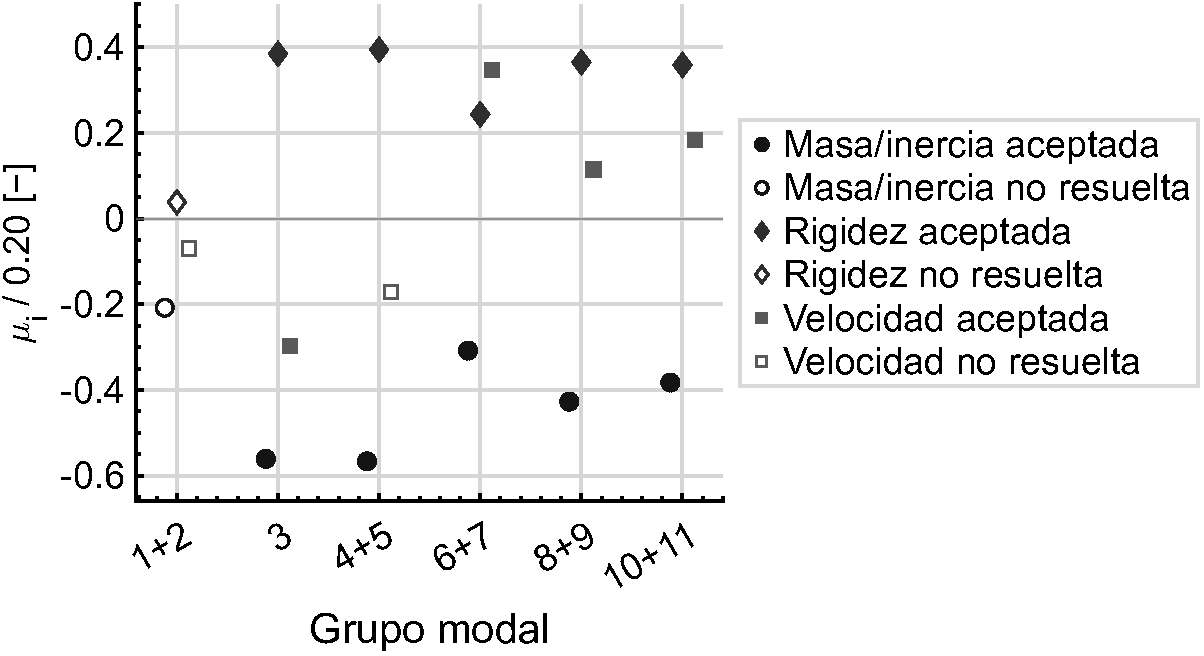
\includegraphics[width=.98\linewidth,height=.40\textheight,keepaspectratio]{figures/actualizacion_20261014/influencia_firmada_grupos.pdf}
\caption{Estimadores originales de Morris, con las etiquetas reales de los grupos. Se representa $\mu_i/0.20$; círculos para masa/inercia, diamantes para rigidez y cuadrados para velocidad. Los símbolos llenos indican influencia aceptada y los vacíos, no resuelta. El grupo 12 permanece excluido. La figura nueva conserva los datos del Morris y utiliza el estilo monocromático autorizado.}\label{fig:sentidos}
\end{figure}


La masa/inercia tiene signo negativo en todos los grupos aceptados y la rigidez, positivo. La velocidad tiene mayor magnitud relativa en 6+7, mientras que reduce la frecuencia de 3. El giro, por tanto, no produce un aumento universal de todas las frecuencias. La comparación de magnitudes es entre factores con el mismo ancho relativo y dentro de cada respuesta.

Para 10+11, la frecuencia nominal es $f_{d,0}=1.22543$ Hz y
\begin{equation}
\overline c_\rho=-0.38266,\qquad
\overline c_K=0.35860,\qquad
\overline c_\Omega=0.18389.
\end{equation}
Como orientación de magnitud, al aplicar $\Delta f_d\simeq f_{d,0}\overline c_i\Delta\xi_i$ a un aumento de 1\pct\ del factor se obtiene:
\begin{center}\small
\begin{tabular}{lrr}
\toprule Factor que aumenta & Cambio relativo orientativo & Cambio orientativo [Hz] \\ \midrule
Masa/inercia & -0.383\,\pct & -0.00469 \\
Rigidez & +0.359\,\pct & +0.00439 \\
Velocidad & +0.184\,\pct & +0.00225 \\

\bottomrule
\end{tabular}
\end{center}
Estos valores son ejemplos calculados a partir de secantes medias; \emph{no son nuevos casos a 1\pct\ ni predicciones locales certificadas}. Los signos y magnitudes son coherentes con las derivadas aceptadas de la primera etapa en el mismo grupo.

\subsection{Intervalos observados de frecuencia}
\begin{center}\small
\begin{tabular}{lrrr}
\toprule Respuesta & Nominal [Hz] & Mínimo observado [Hz] & Máximo observado [Hz] \\ \midrule
1+2 & 0.158 & 0.152 & 0.162 \\
3 & 0.231 & 0.205 & 0.263 \\
4+5 & 0.409 & 0.365 & 0.457 \\
6+7 & 0.587 & 0.536 & 0.641 \\
8+9 & 0.844 & 0.771 & 0.923 \\
10+11 & 1.225 & 1.116 & 1.342 \\

\bottomrule
\end{tabular}
\end{center}
Los extremos reúnen cambios simultáneos de los tres factores en los vértices calculados. No son intervalos de confianza ni extremos demostrados de todo el dominio continuo. En 10+11 se observaron 1.116--1.342 Hz. El rango observado en 1+2 existe, aunque sus influencias individuales no pasaron el filtro de ruido: observar variación y atribuirla con resolución suficiente son afirmaciones distintas.

\section{Qué mecanismos físicos respaldan las tendencias}
\subsection{Masa y rigidez: intuición y comprobación}
Como analogía, un oscilador escalar de masa $m$ y rigidez $k$ tiene $f=(2\pi)^{-1}\sqrt{k/m}$, de donde
\begin{equation}
\frac{\Delta f}{f}\simeq\frac{1}{2}\frac{\Delta k}{k}-\frac{1}{2}\frac{\Delta m}{m}.
\end{equation}
La relación explica por qué aumentar masa suele reducir frecuencia y aumentar rigidez suele elevarla. Es una analogía para interpretar signos; no sustituye el aerogenerador multicuerpo en rotación ni establece coeficientes exactos de $\pm0.5$ para sus factores.

En el modelo, $\xi_\rho$ cambia inercia traslacional y rotacional de palas, peso y contribuciones asociadas al giro; también cambia el equilibrio. $\xi_K$ modifica conjuntamente las rigideces axial, de cortante, torsional y de flexión. Los coeficientes observados incluyen acoplamiento con torre, góndola, cubo y conexiones, cuya masa y rigidez no se escalan en esta campaña. Por eso el efecto no se reduce a reemplazar toda la masa o toda la rigidez del sistema.

\begin{figure}[htbp]
\centering
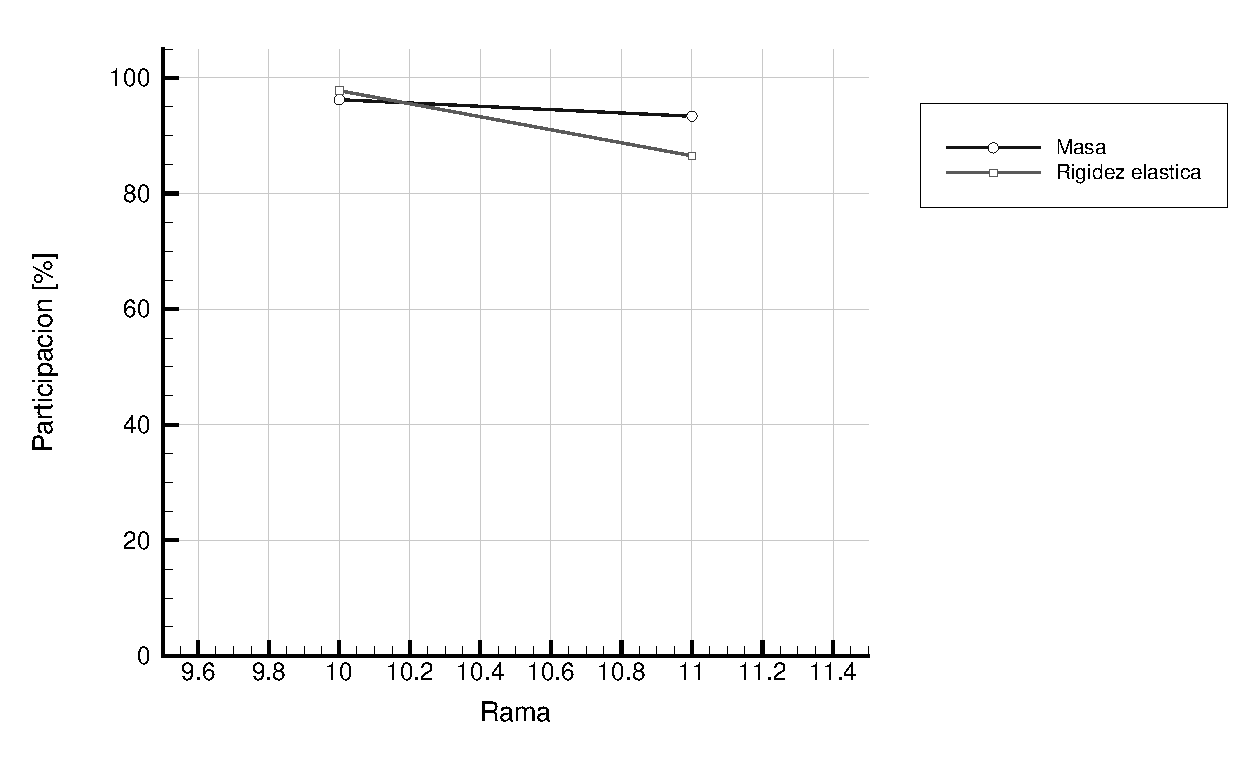
\includegraphics[width=.96\linewidth,height=.40\textheight,keepaspectratio]{figures/tecplot/morris_participaciones.pdf}
\caption{Comprobación mecánica independiente en la referencia de la primera etapa. Las palas aportan aproximadamente 96.2 y 93.4\pct\ de la forma cuadrática de masa, y 97.8 y 86.5\pct\ de la forma cuadrática elástica de las ramas 10 y 11. Se utilizan masa y rigidez elástica de referencia; no se representa toda la energía del sistema en rotación.}
\label{fig:participaciones}
\end{figure}


Para interpretar las participaciones de la figura~\ref{fig:participaciones}, sea $\boldsymbol\phi$ una forma nominal y $\mathsf M_c$ la contribución de masa del componente $c$. Su participación de referencia se obtiene de $\boldsymbol\phi^{\mathsf H}\mathsf M_c\boldsymbol\phi$ dividida por la suma de las contribuciones; $\mathsf H$ indica transposición conjugada. Se procede de forma análoga con la rigidez elástica de referencia. La presencia predominante de palas en 10 y 11 respalda la sensibilidad a sus propiedades. Estas participaciones no separan cuantitativamente todos los mecanismos de la tangente rotacional.

\subsection{Giro: competencia de contribuciones}
El incremento de velocidad modifica efectos giroscópicos proporcionales a $\Omega$, contribuciones inerciales y de transporte, términos proporcionales a $\Omega^2$, el equilibrio y las derivadas de las restricciones y de la transformación de coordenadas. La matriz de velocidad y la tangente intervienen simultáneamente en el problema cuadrático; no basta imaginar una rigidez adicional positiva.

El signo negativo observado en 3 y positivo en 6+7, 8+9 y 10+11 es evidencia de que la respuesta al giro depende del grupo. La hipótesis mecánica compatible con la formulación es una competencia de contribuciones cuya proyección modal cambia de una rama a otra. El cribado no identifica cuánto aporta individualmente cada término; esa separación requeriría un diagnóstico adicional del modelo existente.

\subsection{Compensación parcial entre masa y rigidez}
A velocidad fija, la orientación media del grupo 10+11 sugiere
\begin{equation}
\frac{\Delta f_d}{f_{d,0}}\simeq-0.38266\Delta\xi_\rho+0.35860\Delta\xi_K.
\end{equation}
Una cancelación aproximada de estas secantes daría $\Delta\xi_K\simeq1.067\Delta\xi_\rho$. Esta proporción es una \emph{hipótesis de compensación para comprobar}, no una ley válida para todos los puntos. Diferentes propiedades podrían producir frecuencias similares: ajustar solo una frecuencia puede dejar ambigüedad entre masa y rigidez.

\begin{figure}[htbp]
\centering
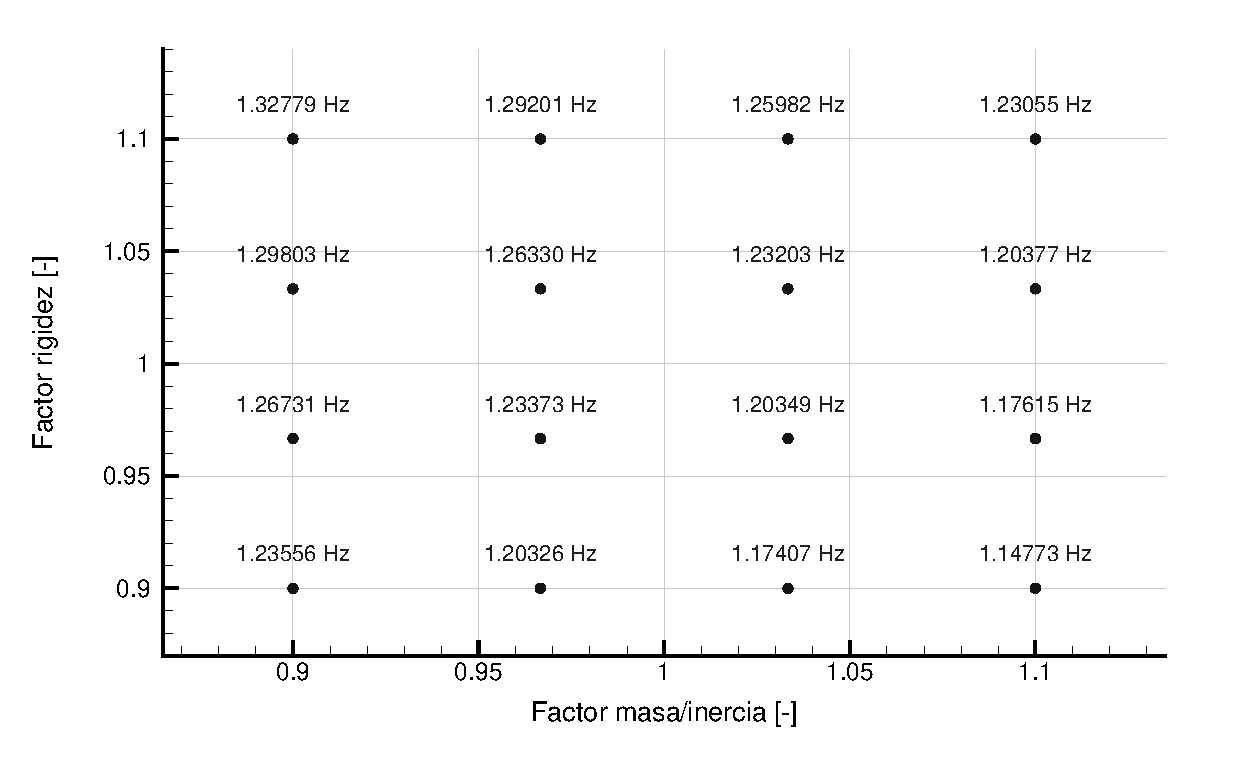
\includegraphics[width=.96\linewidth,height=.40\textheight,keepaspectratio]{figures/tecplot/morris_dominio.pdf}
\caption{Dieciséis combinaciones evaluadas a velocidad fija de 12.4 rpm. Cada punto y su etiqueta corresponden a una frecuencia media del grupo 10+11 almacenada. No se interpolan frecuencias entre puntos. Aumentar masa/inercia y aumentar rigidez producen efectos opuestos; la compensación diagonal es parcial.}\label{fig:dominio}
\end{figure}


La diagonal de la figura~\ref{fig:dominio} muestra frecuencias próximas al aumentar conjuntamente masa y rigidez. Por ejemplo, las esquinas de factores iguales $(0.90,0.90)$ y $(1.10,1.10)$ dan aproximadamente 1.236 y 1.231 Hz a 12.4 rpm. Los valores son cercanos, pero distintos; la compensación no es exacta. Sería útil contrastar más de una frecuencia, formas modales u otros indicadores al identificar propiedades.

\section{Por qué se aceptan unos resultados y otros no}
Se evalúan tres preguntas numéricas: ¿se sigue la misma respuesta modal?, ¿el efecto supera el ruido?, ¿el estimador se estabiliza al aumentar trayectorias? El éxito del solver no garantiza por sí solo las tres condiciones. En esta campaña, las formas y grupos cerrados se conservaron; el grupo abierto asociado a 12 se rechazó.

\subsection{Ruido y señal}
Sea $\eta$ la máxima diferencia de una respuesta observada entre controles: repetición nominal, tolerancia QEP más estricta y solución directa frente a continuación, en el nominal y dos esquinas. Se asigna la envolvente empírica por efecto
\begin{equation}
b_i^{(j)}=\frac{2\eta}{|\Delta x_i^{(j)}|s_y},\qquad
\overline b_i=\frac{1}{r}\sum_j b_i^{(j)}.
\end{equation}
La media absoluta debe satisfacer $\mu_i^*\geq10\overline b_i$. La envolvente no es una cota rigurosa de error en todo el dominio. La comparación con continuación es relevante porque diferencias pequeñas del equilibrio y la tangente pueden afectar indicadores aunque el residuo de equilibrio sea reducido.

\begin{figure}[htbp]
\centering
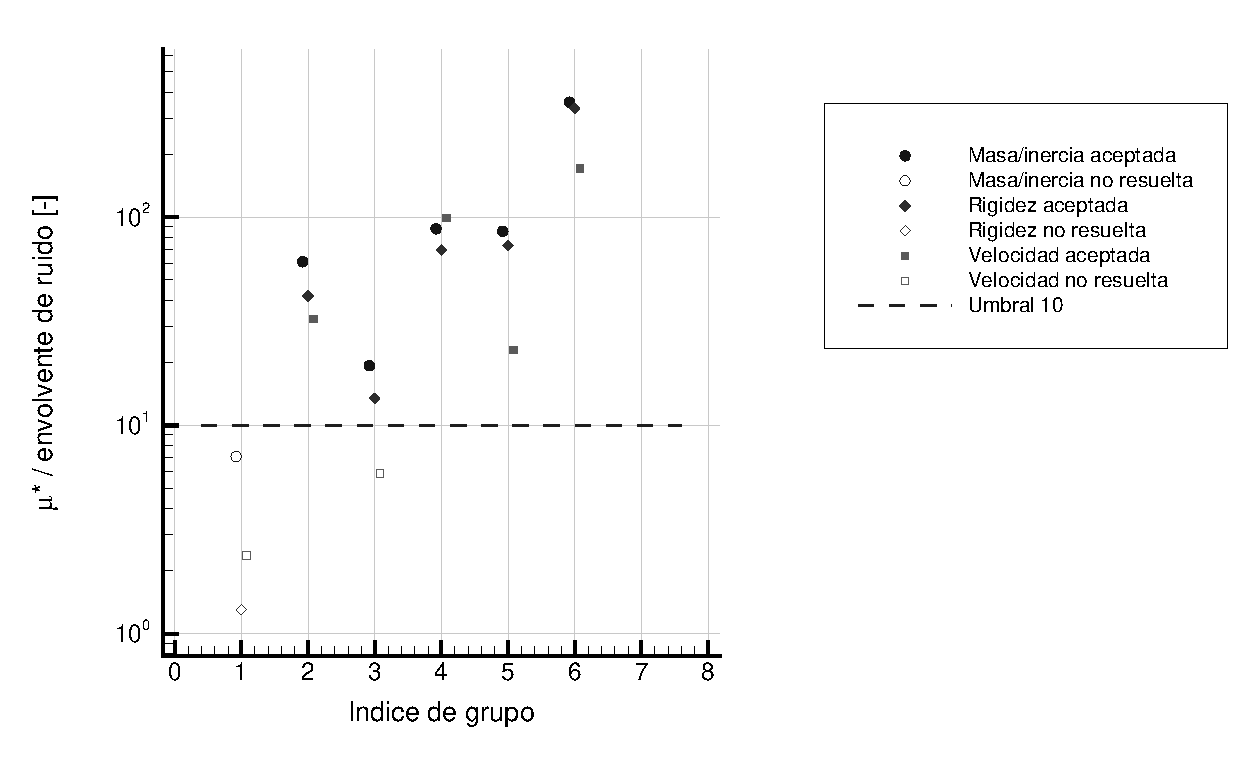
\includegraphics[width=.96\linewidth,height=.40\textheight,keepaspectratio]{figures/tecplot/morris_ruido.pdf}
\caption{Influencia frente a la envolvente empírica de ruido, en escala logarítmica. Se conserva el orden de grupos de la figura de secantes; la línea horizontal indica el umbral de aceptación 10. Los marcadores vacíos permanecen no resueltos. La estabilización de una media no basta para aceptarla.}\label{fig:ruido}
\end{figure}


Por ejemplo, para masa/inercia en 1+2 el cociente señal/ruido es 7.09 y, para velocidad en 4+5, 5.88: ambos quedan bajo el umbral 10. No se publican como influencias aceptadas, aunque sus estimadores cambian menos de 1\pct\ entre veinte y cuarenta trayectorias. Esto evita confundir una estimación repetible con una estimación suficientemente resuelta.

\subsection{Estabilización con el número de trayectorias}
\begin{figure}[htbp]
\centering
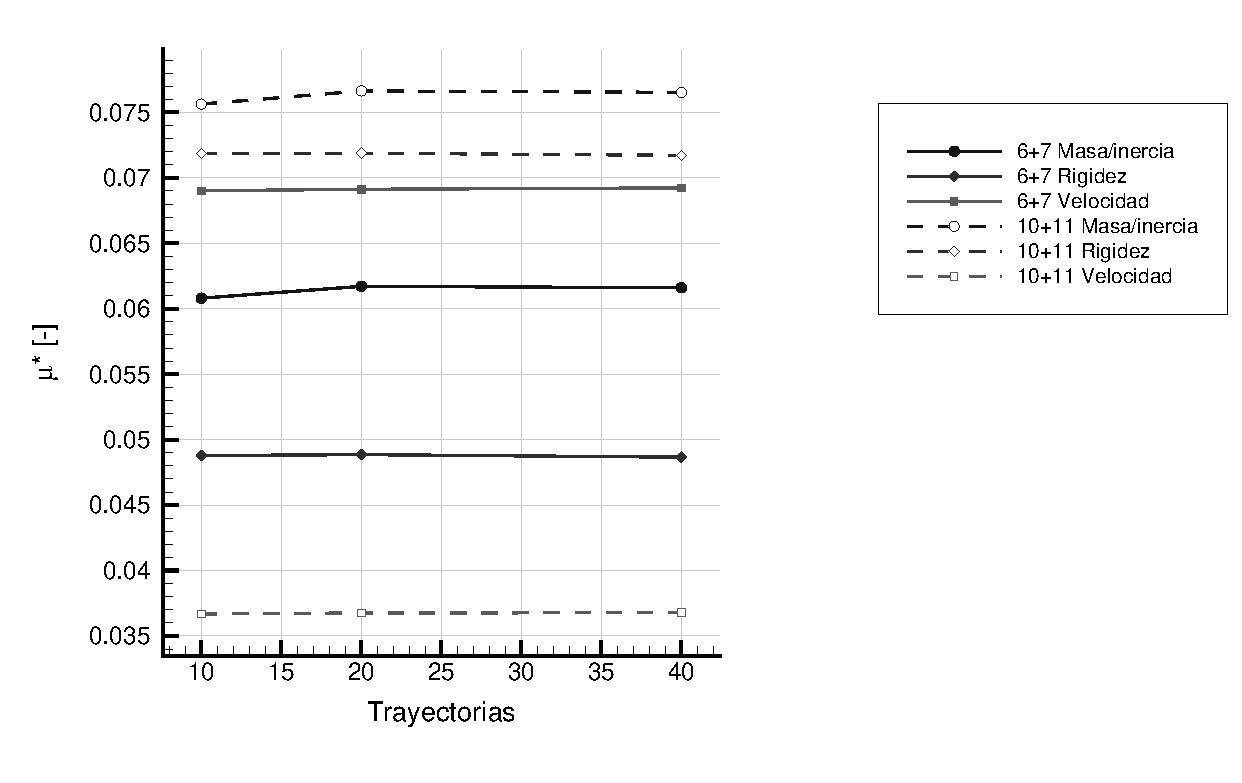
\includegraphics[width=.96\linewidth,height=.40\textheight,keepaspectratio]{figures/tecplot/morris_convergencia.pdf}
\caption{Estabilización de estimadores de los grupos 6+7 y 10+11 con prefijos de 10, 20 y 40 trayectorias del mismo diseño. Los símbolos distinguen factores y la leyenda identifica cada grupo. Las líneas unen prefijos calculados y no prueban convergencia asintótica.}\label{fig:convergencia}
\end{figure}


El máximo cambio relativo de $\mu_i^*$ entre veinte y cuarenta, entre los catorce indicadores aceptados, fue 0.80\,\pct. El umbral fijado era 10\pct. El orden de influencia se conserva en los grupos mostrados. Este resultado apoya la suficiencia del cribado para estas respuestas; no demuestra convergencia espacial de las sensibilidades en rotación ni elimina la dependencia de la malla numérica de Morris.

Los máximos residuos de equilibrio y del QEP en norma dual de masa fueron $9.94\times10^{-9}$ y $4.05\times10^{-9}$, respectivamente. Esta norma reúne fuerzas y momentos con una escala dimensional compatible. Las 170 evaluaciones convergieron y pasaron 17 pruebas del módulo. La regresión histórica de 155 pruebas se conserva como evidencia anterior; no se presenta como una nueva ejecución. Las 148 fuentes físicas MATLAB anteriores permanecieron intactas.

\section{Qué significa la dispersión aceptada}
\begin{figure}[htbp]
\centering
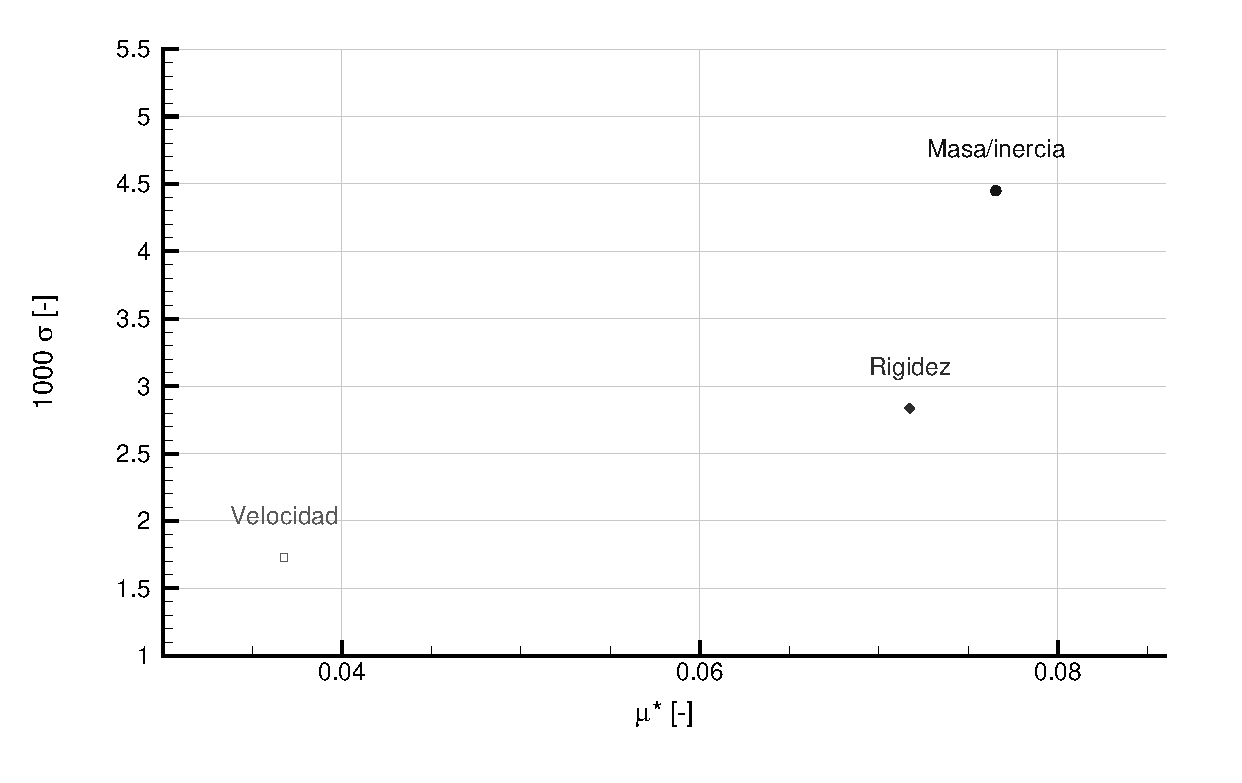
\includegraphics[width=.96\linewidth,height=.40\textheight,keepaspectratio]{figures/tecplot/morris_dispersion.pdf}
\caption{Influencia y dispersión de efectos elementales en el grupo 10+11. Los puntos llenos superan los controles de ruido y estabilización de $\sigma_i$; el punto vacío no. El eje vertical está multiplicado por $10^3$. Esta dispersión describe los efectos elementales, no una distribución física de frecuencias ni una probabilidad de fallo.}
\label{fig:dispersion}
\end{figure}


La dispersión indica que el efecto elemental cambia según el punto donde se evalúa. Puede reunir curvatura respecto del propio factor, dependencia de los otros factores e influencia numérica. Morris no separa estas causas. Para $\sigma_i$, la envolvente propagada es $b_{\sigma,i}=[\sum_j(b_i^{(j)})^2/(r-1)]^{1/2}$; se exige $\sigma_i\geq10b_{\sigma,i}$ y estabilización al 10\pct.

\begin{center}\small
\begin{tabular}{lrrrr}
\toprule Factor; grupo 10+11 & $\sigma_i$ & $\sigma_i/b_{\sigma,i}$ & Cambio 20--40 & Aceptado \\ \midrule
Masa/inercia & 0.00445 & 20.52 & 6.31\,\pct & Sí \\
Rigidez & 0.00283 & 13.07 & 8.22\,\pct & Sí \\
Velocidad & 0.00173 & 7.97 & 14.94\,\pct & No \\

\bottomrule
\end{tabular}
\end{center}
La dispersión de masa/inercia y rigidez supera el ruido y cambia aproximadamente 6.31\pct\ y 8.22\pct, respectivamente. La de velocidad tiene cociente 7.97 y no supera el filtro de ruido. No puede afirmarse que el giro sea exactamente lineal o independiente de los otros factores por ese rechazo. Tampoco puede afirmarse que las dos dispersiones aceptadas demuestren, por sí solas, una interacción específica.








% BEGIN COMPLEMENT 20261014
\clearpage
\section{Comprobación complementaria de la rejilla y de los efectos combinados}
\subsection{Cobertura, controles y conservación del modelo}
La rejilla de cuatro niveles y tres factores contiene $4^3=64$ combinaciones. Morris había visitado 58 combinaciones distintas. Se resolvieron las seis faltantes y tres controles: QEP más estricto y continuación en uno de esos puntos, y repetición nominal. Se conservaron los casos de Morris y sus estimadores. Las nueve evaluaciones nuevas tomaron 77.49 s de solve, bajo un límite operacional de 300 s. La campaña modal global reúne así 170 evaluaciones originales y nueve complementarias, con 64 puntos de rejilla distintos.

Se verificaron las 175 huellas de fuentes de la campaña original. Los grupos históricos se conservan y sus formas pasan las comprobaciones correspondientes. La rama 12 continúa abierta frente a ramas fuera del conjunto seguido y queda excluida. Los rangos físicos, propiedades vinculadas y formulación permanecen iguales. La continuación y el QEP estricto en un nuevo punto no aumentaron la envolvente de frecuencia de 10+11: $\eta=8.7456\times10^{-5}$ Hz. La diferencia máxima de sus controles nuevos fue $1.0613\times10^{-5}$ Hz.

Las medias de secantes de extremos conservan el orden de influencia de los cinco grupos principales. Sus pasos y ponderaciones difieren de Morris, de modo que no son estimadores idénticos ni derivadas infinitesimales. En 1+2, la media absoluta de secantes de masa de extremo tiene cociente señal/ruido 10.41, cercano al umbral 10; solo once de sus dieciséis comparaciones individuales superan ese umbral. Este resultado marginal no cambia retrospectivamente la ausencia de aceptación de su estimador Morris.

\subsection{Compensación parcial a las cuatro velocidades}
Se examina la diagonal $\xi_\rho=\xi_K$ a 10.8, 11.6, 12.4 y 13.2 rpm. El cambio entre factores iguales 0.90 y 1.10 es de aproximadamente 0.00495--0.00519 Hz, equivalente a 0.404--0.423\pct\ de $f_{d,0}$ de 10+11. Cada curva de la figura usa como origen su propio punto diagonal 0.90. La cercanía de frecuencias apoya una compensación parcial, pero no una identidad válida para toda la respuesta. La identificación de propiedades necesita otras frecuencias, formas u observaciones.
\begin{figure}[htbp]\centering
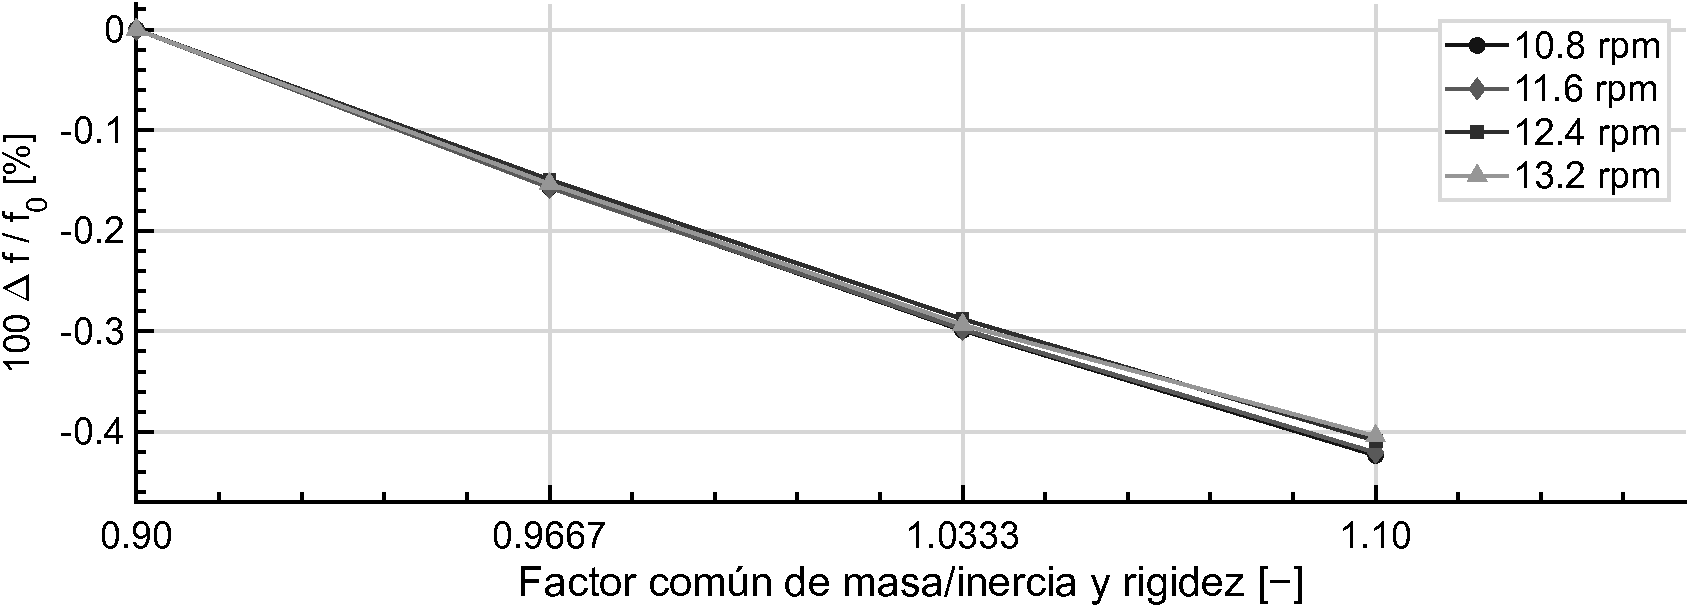
\includegraphics[width=.92\linewidth,height=.37\textheight,keepaspectratio]{figures/actualizacion_20261014/compensacion_rejilla.pdf}
\caption{Cambios de frecuencia de 10+11 a lo largo de la diagonal masa--rigidez, medidos respecto del punto 0.90 de cada velocidad y normalizados por la frecuencia nominal fija. Se muestran únicamente valores calculados de la rejilla; las líneas conectan esos valores.}\label{fig:compensacion-rejilla}
\end{figure}
\FloatBarrier

\subsection{Contraste rectangular para distinguir no aditividad}
Para dos factores $i,j$, con el tercero fijo, se calcula el contraste de sus extremos:
\begin{equation}
I_{ij}=f_{++}-f_{+-}-f_{-+}+f_{--}.
\end{equation}
Los signos indican factores 1.10 y 0.90. Si la respuesta fuera una suma de funciones separadas de los dos factores, el contraste sería cero, incluso si dichas funciones tuvieran curvatura individual. Un contraste resuelto evidencia no aditividad de esta respuesta en esos puntos. No atribuye un mecanismo concreto a un término del operador ni cuantifica un porcentaje de varianza.

La envolvente propagada es $b_I=4\eta$, por los cuatro términos del contraste. Se exige $|I_{ij}|\geq10b_I$, además de seguimiento válido. La cota continúa siendo empírica. Para 10+11 se obtiene:
\begin{center}\small
\begin{tabular}{lrrl}\toprule
Par & $|I_{ij}|$ [Hz] & $|I_{ij}|/b_I$ & Interpretación \\ \midrule
Masa--rigidez & 0.00926--0.00940 & 26.47--26.87 & Resuelto \\
Masa--velocidad & 0.00356--0.00362 & 10.17--10.34 & Marginal sobre el umbral \\
Rigidez--velocidad & 0.00331--0.00342 & 9.47--9.77 & No resuelto \\
\bottomrule\end{tabular}
\end{center}
Masa--rigidez presenta contraste negativo en las cuatro velocidades. El incremento de rigidez tiene menor efecto de frecuencia al aumentar masa, de forma compatible con la dependencia conjunta de rigidez e inercia. La afirmación se limita al contraste observado, no a una separación causal de todos los operadores. Masa--velocidad supera por poco el umbral y requiere cautela. Rigidez--velocidad permanece sin resolución suficiente; no se infiere ausencia de interacción.
\begin{figure}[htbp]\centering
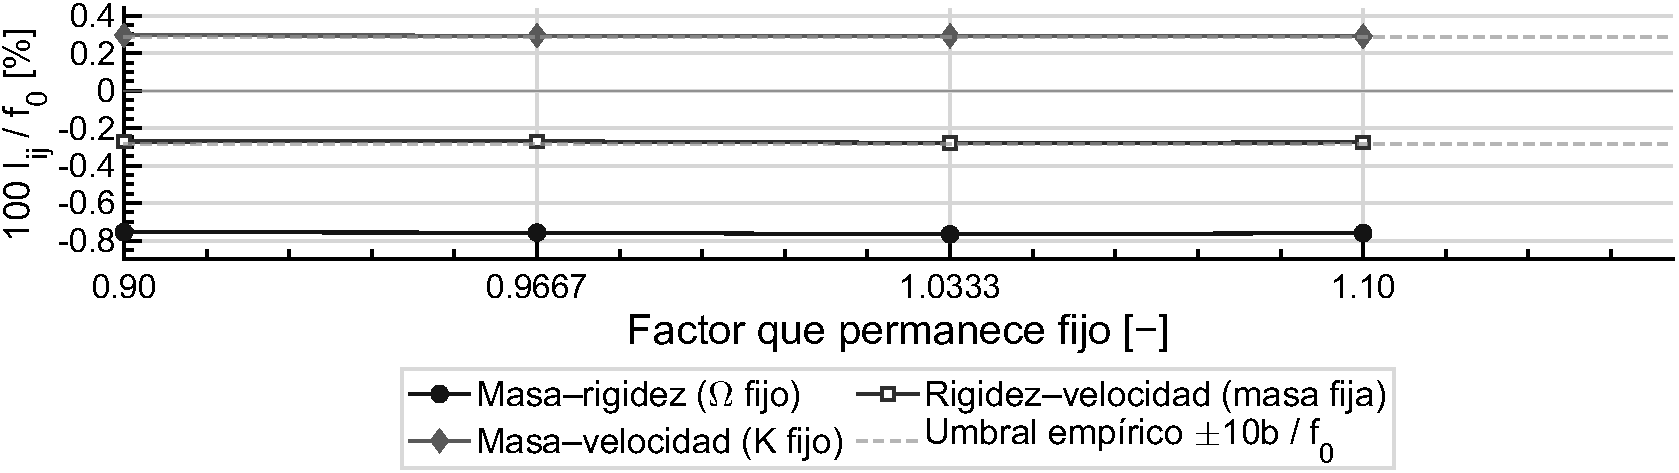
\includegraphics[width=.98\linewidth,height=.38\textheight,keepaspectratio]{figures/actualizacion_20261014/contrastes_interaccion.pdf}
\caption{Contrastes de extremos en 10+11, normalizados por $f_{d,0}$. Cada curva deja fijo un factor diferente, identificado en la leyenda. Los símbolos llenos superan el umbral empírico y los vacíos no. Las líneas discontinuas muestran $\pm10b_I/f_{d,0}$ en porcentaje.}\label{fig:contrastes-interaccion}
\end{figure}
\FloatBarrier

\subsection{Curvatura individual y límites de esta comprobación}
En pasos igualmente espaciados se calcula $C_i=f_{i+1}-2f_i+f_{i-1}$. En 10+11, seis de los 32 contrastes de masa/inercia superan diez veces la envolvente $4\eta$. Ninguno de los 32 contrastes de rigidez o de velocidad supera ese filtro. Por tanto, la evidencia adicional resuelve curvatura de masa en ciertos puntos y no aditividad masa--rigidez; las restantes ausencias de resolución no prueban linealidad.

El contraste masa--velocidad es un indicador diferente de $\sigma_\Omega$ de Morris, cuya aceptación original sigue siendo negativa. La rejilla completa verifica todos sus 64 puntos discretos, sin certificar extrema o monotonicidad del dominio continuo, convergencia espacial en operación ni incertidumbre probabilística. Sus tablas guardan también todos los indicadores que no superan el filtro.

La licencia de Tecplot vencida impidió exportaciones nuevas. El autor autorizó el 14 de octubre utilizar las figuras ya generadas y producir las restantes con el mismo formato y estilo. Se exportaron tres figuras nuevas y cuatro adaptaciones de legibilidad para la presentación con MATLAB R2026a, en escala de grises, fondo blanco y PDF vectorial. Su catálogo registra motor, datos y procedencia. Las figuras anteriores conservan su procedencia Tecplot.
% END COMPLEMENT 20261014

\section{Estabilidad, alcance y decisiones para continuar}
Las partes reales de los dieciséis representantes modales retornados por evaluación fueron negativas; la mayor observada fue $-0.01238$ s$^{-1}$. Bajo los operadores congelados, esto es compatible con decaimiento de esas perturbaciones modales seleccionadas. El espectro es parcial y no se calcula estabilidad periódica de Floquet: el dato no demuestra estabilidad de toda la turbina ni de todas las velocidades posibles. La sensibilidad de un centroide de crecimiento tampoco sustituye el examen de cada raíz.

La verificación espacial previa se realizó con rotor detenido, y la convergencia temporal corresponde al benchmark sísmico local anterior. No verifican automáticamente las sensibilidades globales en rotación. Esta etapa utiliza propiedades heredadas sin calibración experimental y tres factores elegidos; no estudia incertidumbre probabilística ni sensibilidad sísmica global.

Las siguientes decisiones científicas se pueden discutir con el asesor:
\begin{enumerate}
\item Obtener fuentes para rangos físicos y propiedades de palas, conexiones y apoyo. Esto permitiría pasar de escenarios a incertidumbre justificada.
\item Priorizar la convergencia espacial de las respuestas y sensibilidades con rotor en operación, conservando restricciones y seguimiento modal.
\item Ampliar la identificación masa--rigidez con otras respuestas y formas, partiendo de los contrastes ya comprobados en 10+11.
\item Definir si el alcance del artículo será sensibilidad a azimut fijo o si se requiere un estudio periódico adicional para afirmaciones de estabilidad.
\end{enumerate}
La comprobación de la rejilla y los contrastes finitos anteriores ya se ejecutaron. Los restantes puntos son propuestas científicas para acordar; no se han ejecutado campañas de refinamiento en operación ni estabilidad periódica.

\section{Guía breve para la reunión}
\paragraph{Apertura.} Se auditó y conservó el modelo existente, se implementó sensibilidad total con nuevo equilibrio y se pasó de derivadas locales a un cribado Morris sobre escenarios aprobados. La implementación conserva trazabilidad y rechaza resultados sin resolución suficiente.
\paragraph{Resultado principal.} La influencia depende del grupo: masa/inercia domina cuatro respuestas y velocidad domina 6+7 entre los tres factores. La frecuencia de 3 disminuye al aumentar giro; las de tres grupos superiores aumentan. Se usa la figura~\ref{fig:sentidos} para mostrar simultáneamente dirección y magnitud.
\paragraph{Mecanismo respaldado.} La participación nominal predominante de palas en 10 y 11 apoya la sensibilidad a sus propiedades. Las figuras~\ref{fig:dominio} y~\ref{fig:compensacion-rejilla} muestran la compensación parcial; los contrastes de la figura~\ref{fig:contrastes-interaccion} resuelven no aditividad masa--rigidez en 10+11. La separación exacta de contribuciones del giro sigue abierta.
\paragraph{Confianza y límite.} Catorce influencias y dos dispersiones superan los filtros. Los estimadores de influencia cambian menos de 1\pct\ al duplicar veinte a cuarenta trayectorias. Las figuras~\ref{fig:ruido} y~\ref{fig:dispersion} muestran por qué otros indicadores permanecen no resueltos. Esta evidencia es numérica y de azimut fijo.
\paragraph{Decisión a pedir.} Acordar cuál será la siguiente contribución: rangos físicos, convergencia espacial en operación, identificación con múltiples respuestas o extensión periódica. La elección debe estar ligada a la afirmación científica que se quiera sostener en el artículo y la tesis.

\appendix
\section{Valores de los catorce indicadores aceptados}
\begin{center}\small
\begin{tabular}{llrrr}
\toprule Factor & Grupo & $\mu_i$ & $\mu_i^*$ & $\sigma_i$ \\ \midrule
Masa/inercia & 3 & -0.11221 & 0.11221 & 0.01052 \\
Masa/inercia & 4+5 & -0.11335 & 0.11335 & 0.00670 \\
Masa/inercia & 6+7 & -0.06161 & 0.06161 & 0.00398 \\
Masa/inercia & 8+9 & -0.08546 & 0.08546 & 0.00495 \\
Masa/inercia & 10+11 & -0.07653 & 0.07653 & 0.00445 \\
Rigidez & 3 & +0.07695 & 0.07695 & 0.00652 \\
Rigidez & 4+5 & +0.07886 & 0.07886 & 0.00368 \\
Rigidez & 6+7 & +0.04866 & 0.04866 & 0.00235 \\
Rigidez & 8+9 & +0.07296 & 0.07296 & 0.00291 \\
Rigidez & 10+11 & +0.07172 & 0.07172 & 0.00283 \\
Velocidad & 3 & -0.05952 & 0.05952 & 0.00726 \\
Velocidad & 6+7 & +0.06923 & 0.06923 & 0.00202 \\
Velocidad & 8+9 & +0.02295 & 0.02295 & 0.00155 \\
Velocidad & 10+11 & +0.03678 & 0.03678 & 0.00173 \\

\bottomrule
\end{tabular}
\end{center}
La aceptación de $\mu_i^*$ en esta tabla no implica aceptación de $\sigma_i$ en todas sus filas. Los controles de dispersión se evalúan por separado. Los números se redondean para lectura; las tablas CSV y MAT conservan mayor precisión.

Las figuras históricas se exportaron desde Tecplot y se incluyen como PDF externos. Los datos, macros y paquetes nativos permanecen en su biblioteca. Las figuras nuevas y las adaptaciones para proyección se exportaron desde MATLAB con autorización del autor ante la licencia Tecplot vencida. Las fuentes originales se conservan en morris\_estimators.csv, morris\_sweeps.csv, morris\_vertices.csv, report\_data.json y modal\_energy\_evidence.csv. La comprobación adicional usa grid\_responses.csv y sus tablas de contrastes. No se reemplazaron casos fallidos; los nueve casos nuevos se registran en una campaña separada.

